\documentclass[mathserif,compress]{beamer}\usepackage{graphicx, color}
%% maxwidth is the original width if it is less than linewidth
%% otherwise use linewidth (to make sure the graphics do not exceed the margin)
\makeatletter
\def\maxwidth{ %
  \ifdim\Gin@nat@width>\linewidth
    \linewidth
  \else
    \Gin@nat@width
  \fi
}
\makeatother

\definecolor{fgcolor}{rgb}{0.2, 0.2, 0.2}
\newcommand{\hlnumber}[1]{\textcolor[rgb]{0,0,0}{#1}}%
\newcommand{\hlfunctioncall}[1]{\textcolor[rgb]{0.501960784313725,0,0.329411764705882}{\textbf{#1}}}%
\newcommand{\hlstring}[1]{\textcolor[rgb]{0.6,0.6,1}{#1}}%
\newcommand{\hlkeyword}[1]{\textcolor[rgb]{0,0,0}{\textbf{#1}}}%
\newcommand{\hlargument}[1]{\textcolor[rgb]{0.690196078431373,0.250980392156863,0.0196078431372549}{#1}}%
\newcommand{\hlcomment}[1]{\textcolor[rgb]{0.180392156862745,0.6,0.341176470588235}{#1}}%
\newcommand{\hlroxygencomment}[1]{\textcolor[rgb]{0.43921568627451,0.47843137254902,0.701960784313725}{#1}}%
\newcommand{\hlformalargs}[1]{\textcolor[rgb]{0.690196078431373,0.250980392156863,0.0196078431372549}{#1}}%
\newcommand{\hleqformalargs}[1]{\textcolor[rgb]{0.690196078431373,0.250980392156863,0.0196078431372549}{#1}}%
\newcommand{\hlassignement}[1]{\textcolor[rgb]{0,0,0}{\textbf{#1}}}%
\newcommand{\hlpackage}[1]{\textcolor[rgb]{0.588235294117647,0.709803921568627,0.145098039215686}{#1}}%
\newcommand{\hlslot}[1]{\textit{#1}}%
\newcommand{\hlsymbol}[1]{\textcolor[rgb]{0,0,0}{#1}}%
\newcommand{\hlprompt}[1]{\textcolor[rgb]{0.2,0.2,0.2}{#1}}%

\usepackage{framed}
\makeatletter
\newenvironment{kframe}{%
 \def\at@end@of@kframe{}%
 \ifinner\ifhmode%
  \def\at@end@of@kframe{\end{minipage}}%
  \begin{minipage}{\columnwidth}%
 \fi\fi%
 \def\FrameCommand##1{\hskip\@totalleftmargin \hskip-\fboxsep
 \colorbox{shadecolor}{##1}\hskip-\fboxsep
     % There is no \\@totalrightmargin, so:
     \hskip-\linewidth \hskip-\@totalleftmargin \hskip\columnwidth}%
 \MakeFramed {\advance\hsize-\width
   \@totalleftmargin\z@ \linewidth\hsize
   \@setminipage}}%
 {\par\unskip\endMakeFramed%
 \at@end@of@kframe}
\makeatother

\definecolor{shadecolor}{rgb}{.97, .97, .97}
\definecolor{messagecolor}{rgb}{0, 0, 0}
\definecolor{warningcolor}{rgb}{1, 0, 1}
\definecolor{errorcolor}{rgb}{1, 0, 0}
\newenvironment{knitrout}{}{} % an empty environment to be redefined in TeX

\usepackage{alltt} 
\usepackage{beamerthemeDresden} 
\usepackage[english]{babel}
\usepackage{amsmath,amssymb}
\usepackage[latin1]{inputenc}
\usepackage{palatino}
\usepackage{graphicx}
\usepackage{subfigure}
\usepackage{pgf}
\usepackage{relsize}
\def\beq{\begin{equation}}
\def\eeq{\end{equation}}
\def\bit{\begin{itemize}}
\def\eit{\end{itemize}}
\def\bdm{\begin{displaymath}}
\def\edm{\end{displaymath}}
\def\ben{\begin{enumerate}}
\def\een{\end{enumerate}}
\def\bc{\mathbf{c}}
\def\bd{\mathbf{d}}
\def\bh{\mathbf{h}}
\def\bm{\mathbf{m}}
\def\br{\mathbf{r}}
\def\bs{\mathbf{s}}
\def\bu{\mathbf{u}}
\def\bv{\mathbf{v}}
\def\bw{\mathbf{w}}
\def\bx{\mathbf{x}}
\def\by{\mathbf{y}}
\def\bz{\mathbf{z}}
\def\bA{\mathbf{A}}
\def\bD{\mathbf{D}}
\def\bG{\mathbf{G}}
\def\bI{\mathbf{I}}
\def\bQ{\mathbf{Q}}
\def\bR{\mathbf{R}}
\def\bS{\mathbf{S}}
\def\bV{\mathbf{V}}
\def\bW{\mathbf{W}}
\def\bX{\mathbf{X}}
\def\bY{\mathbf{Y}}
\def\bZ{\mathbf{Z}}
\def\cB{\mathcal{B}}
\def\cF{\mathcal{F}}
\def\cI{\mathcal{I}}
\def\cK{\mathcal{K}}
\def\cU{\mathcal{U}}
\def\bbeta{\mbox{\boldmath $\beta$}}
\def\bepsilon{\mbox{\boldmath $\epsilon$}}
\def\bdelta{\mbox{\boldmath $\delta$}}
\def\bgamma{\mbox{\boldmath $\gamma$}}
\def\bldeta{\mbox{\boldmath $\eta$}}
\def\bphi{\mbox{\boldmath $\phi$}}
\def\bkappa{\mbox{\boldmath $\kappa$}}
\def\blambda{\mbox{\boldmath $\lambda$}}
\def\bmu{\mbox{\boldmath $\mu$}}
\def\bnu{\mbox{\boldmath $\nu$}}
\def\btheta{\mbox{\boldmath $\theta$}}
\def\brho{\mbox{\boldmath $\rho$}}
\def\bDelta{\mbox{\boldmath $\Delta$}}
\def\bLambda{\mbox{\boldmath $\Lambda$}}
\def\bSigma{\mbox{\boldmath $\Sigma$}}
\def\var{\textrm{var}}
\def\cov{\textrm{cov}}
\def\log{\textrm{log}}
\def\median{\textrm{median}}
\def\argmin{\textrm{arg min }}
\def\bzero{\mathbf{0}}
\def\bone{\mathbf{1}}
\def\Poi{\textrm{Poi}}
\def\Unif{\textrm{Unif}}
\def\upp{^\prime}
\def\upi{^{-1}}
\newcommand{\cye}[1]{\color{yellow!70!black}#1}
\newcommand{\cre}[1]{\color{red!70!black}#1}
\newcommand{\cbl}[1]{\color{blue!70!black}#1}
\newcommand{\cgr}[1]{\color{green!70!black}#1}
\IfFileExists{upquote.sty}{\usepackage{upquote}}{}
\begin{document}



\title[]{Block Prediction}

\author[Jay M. Ver Hoef]{Jay Ver Hoef} 

\institute[NOAA National Marine Mammal Lab]
{
	\normalsize National Marine Mammal Lab \\
	NOAA Fisheries \\
	International Arctic Research Center \\
	Fairbanks, Alaska, USA\\
	\vspace{0.1cm}
}
\date[05/17/13]{}
 
\maketitle
 
% very important to use option [fragile] for frames containing code output!
   
%-------------------------------------------------------------------------------
%                        Introduction
%-------------------------------------------------------------------------------

\section{Introduction}
\subsection{}
\begin{frame}[fragile]
\frametitle{Introduction}
	
	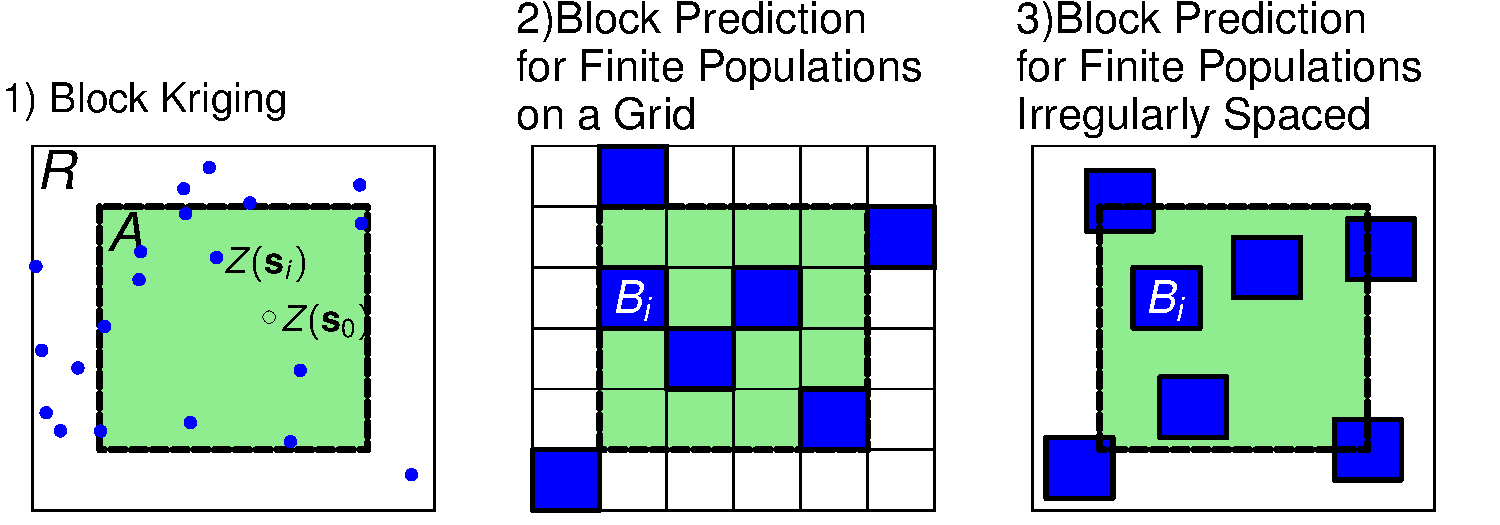
\includegraphics[width=\maxwidth]{figure/Introductory-plot}

\end{frame}

%-------------------------------------------------------------------------------
%                 Block Prediction on a Stream Network
%-------------------------------------------------------------------------------

\begin{frame}[fragile]
\frametitle{Block Prediction on a Stream Network}

	\scriptsize
	Peterson, E.E., Ver Hoef, J.M., Isaak, D.J., Falke, J.A., Fortin, M-J, Jordan, C., McNyset, K., Monestiez, P., Ruesch, A.S., Sengupta, A., Som, N., Steel, A., Theobald, D.M., Torgersen, C.E., Wenger, S.J. 2013. Stream networks in space: concepts, models, and synthesis. {\it Ecology Letters.} doi: 10.1111/ele.12084.
	\begin{center}
		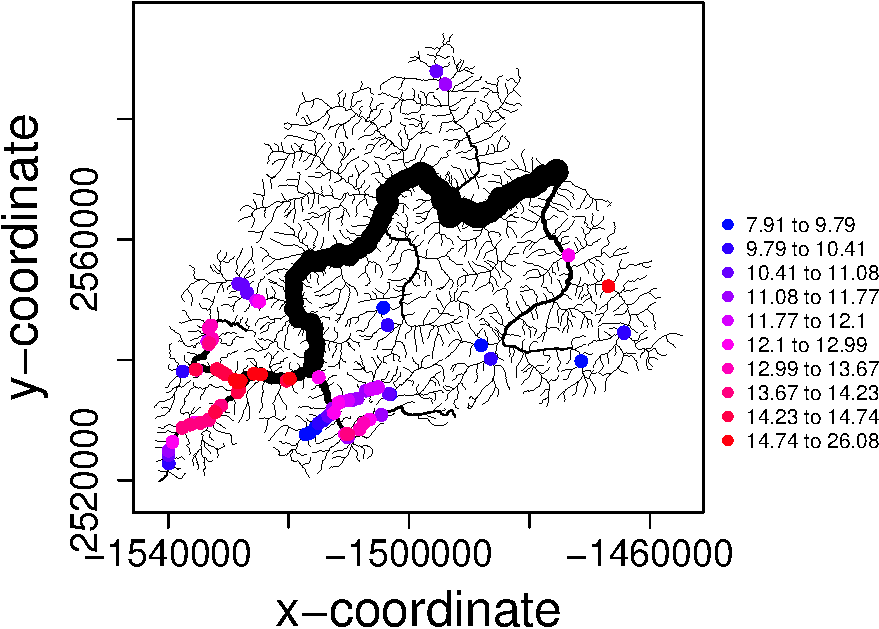
\includegraphics[width=.6\maxwidth]{figure/mf04pTempColoredCrop}
	\end{center}
\end{frame}

%-------------------------------------------------------------------------------
%                 Block Prediction on a Stream Network
%-------------------------------------------------------------------------------

\begin{frame}[fragile]
\frametitle{Block Prediction on a Stream Network}
	
	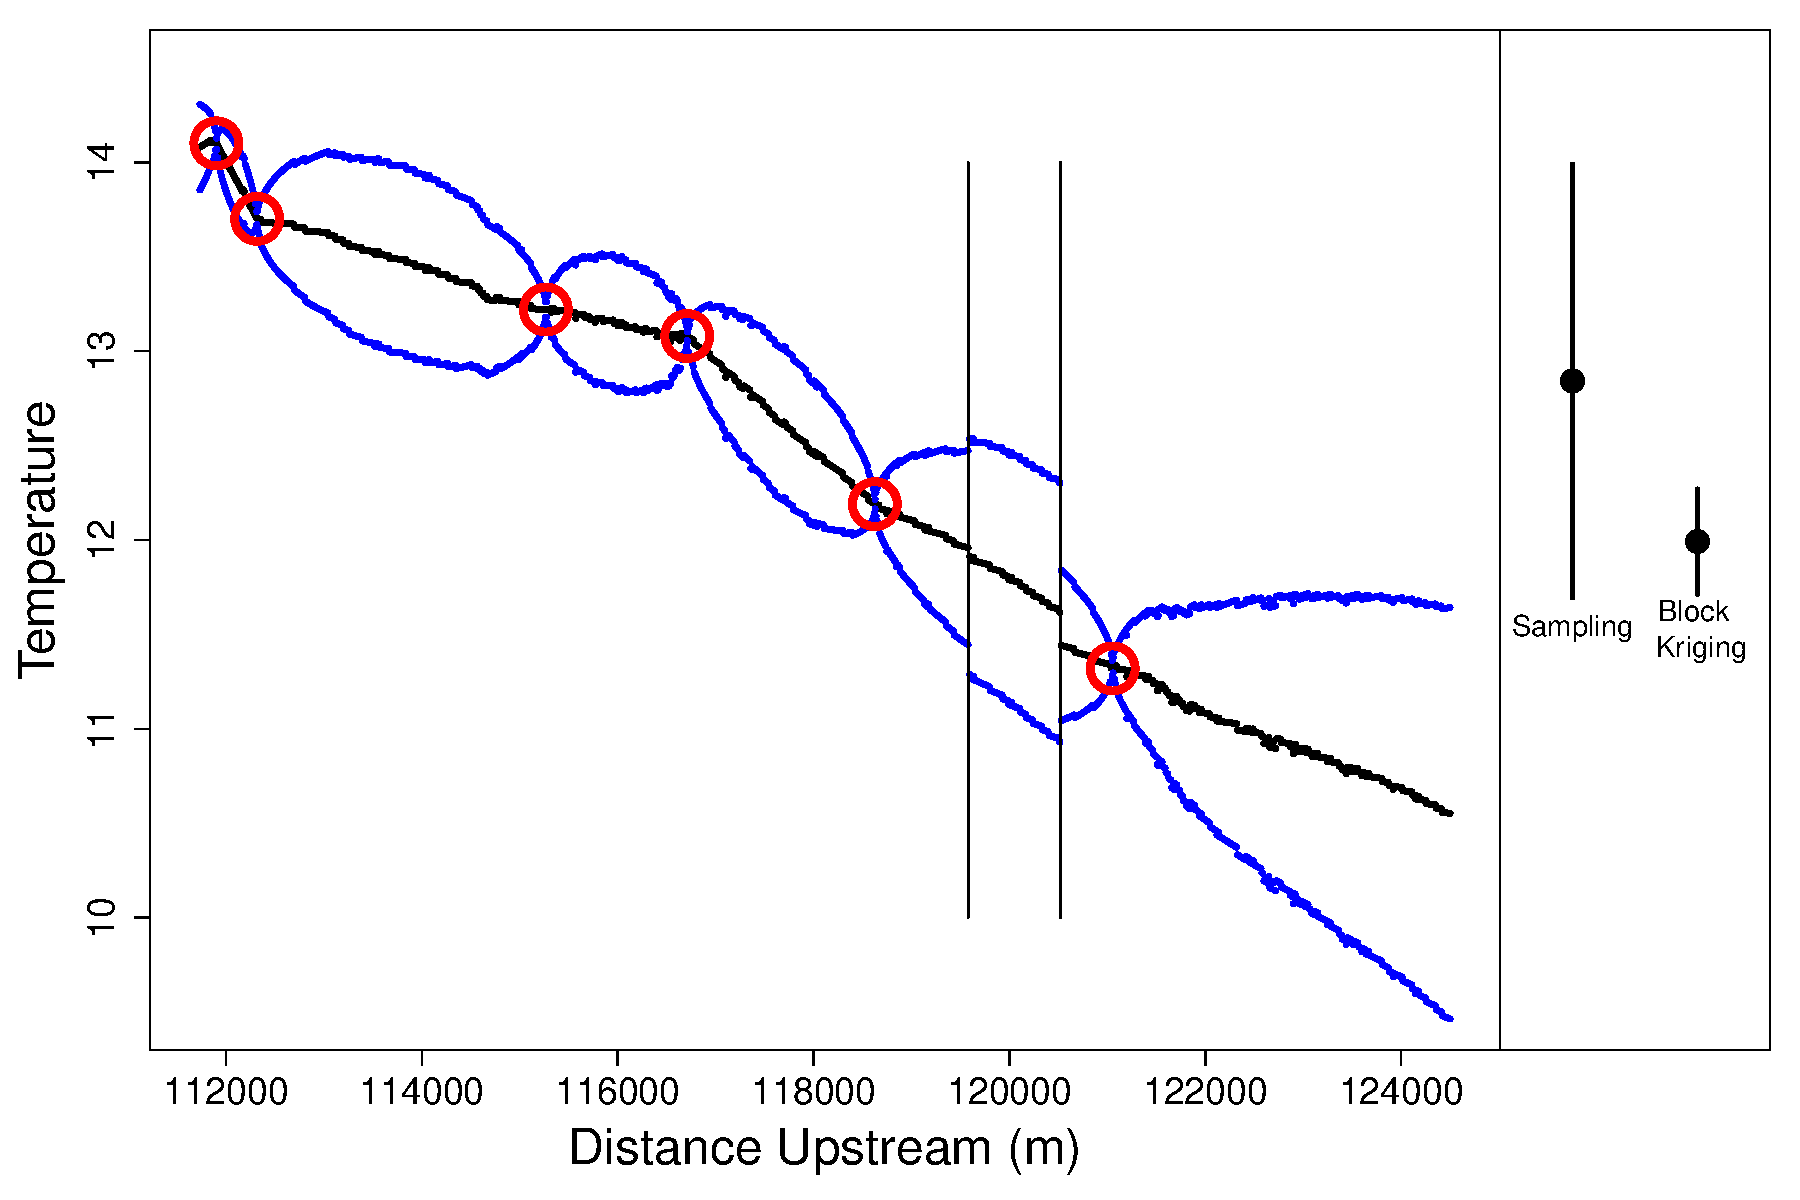
\includegraphics[width=.95\maxwidth]{figure/Figure_BlockKriging120203}

\end{frame}

%-------------------------------------------------------------------------------
%                 Review of BLUP and Point Prediction
%-------------------------------------------------------------------------------

\section{Theory}
\subsection{}
\begin{frame}[fragile]
\frametitle{Review of BLUP and Point Prediction}
	\vspace{-.5cm}
	\[
		\left(\begin{array}{c}
		\bz \\ Z(\bs_0)
		\end{array}\right)	=
		\left(\begin{array}{c}
		\bX \\ \bx(\bs_0)\upp
		\end{array}\right)\bbeta +
		\left(\begin{array}{c}
		\bepsilon \\ \epsilon(\bs_0)
		\end{array}\right)
	\] \\
	\[ 
		\cov\left(\begin{array}{c}
		\bepsilon \\ \epsilon(\bs_0)
		\end{array}\right) = 
		\left(\begin{array}{cc}
		\bSigma & \bc \\ \bc\upp & \sigma_0^2
		\end{array}\right)
	\]
	 \\
	Best Linear Unbiased Prediction (BLUP) (or [Universal] Kriging) \\
	minimize: $\cre{E(\blambda\upp\bz - Z(\bs_0))^2}$ subject to 	$\cre{E[\blambda\upp\bz] = E[Z(\bs_0)] \ \forall \ \bbeta}$. \\
	Unbiasedness $\Rightarrow \bX\upp\blambda = \bx(\bs_0) $ \\		
	$E[\blambda\upp\bepsilon\bepsilon\upp\blambda - 2\blambda\upp\bepsilon \epsilon(\bs_0) + \epsilon(\bs_0)^2] = \blambda\upp\bSigma\blambda - 2\blambda\upp\bc + \sigma_0^2$ \\
	$\frac{\partial}{\blambda\upp} [\blambda\upp\bSigma\blambda - 2\blambda\upp\bc + \sigma_0^2 + 2\bm\upp(\bX\upp\blambda - \bx(\bs_0)] = 0$ \\
	$\frac{\partial}{\bm\upp} [\blambda\upp\bSigma\blambda - 2\blambda\upp\bc + \sigma_0^2 + 2\bm\upp(\bX\upp\blambda - \bx(\bs_0)] = 0$ \\
	$\Rightarrow 2\bSigma\blambda - 2\bc  + 2\bX\bm = 0, \quad \quad \bX\upp\blambda - \bx(\bs_0) = 0$ \\
	 

\end{frame}

%-------------------------------------------------------------------------------
%                 Review of BLUP and Point Prediction
%-------------------------------------------------------------------------------
\begin{frame}[fragile]
\frametitle{Review of BLUP and Point Prediction}

	solve 
	\[
		\left(\begin{array}{cc}
		\bSigma & \bX \\ \bX\upp & \bzero
		\end{array}\right)
		\left(\begin{array}{c}
		\blambda \\ \bm
		\end{array}\right) =
		\left(\begin{array}{c}
		\bc \\ \bx(\bs_0)
		\end{array}\right)
	\]

	$\bSigma\blambda - \bc  + \bX\bm = 0 \Rightarrow \blambda = \bSigma\upi(\bc - \bX\bm)$ \\
	$\bX\upp\blambda - \bx(\bs_0) = 0 \Rightarrow \bX\upp\bSigma\upi(\bc - \bX\bm) = \bx(\bs_0)$ \\
	$\Rightarrow \bm = (\bX\upp\bSigma\upi\bX)\upi(\bX\upp\bSigma\upi\bc - \bx(\bs_0))$
	$\Rightarrow \blambda = \bSigma\upi(\bc + \bX(\bX\upp\bSigma\upi\bX)\upi(\bx(\bs_0) - \bX\upp\bSigma\upi\bc))$ \\
	\vspace{.5cm}
	$ \cre{\hat{Z}(\bs_0) = \blambda\upp\bz}, \quad \cre{\var(\hat{Z}(\bs_0)) = \blambda\upp\bSigma\blambda - 2\blambda\upp\bc + \sigma_0^2}$

\end{frame}

%-------------------------------------------------------------------------------
%                 Alternative Formulas
%-------------------------------------------------------------------------------

\begin{frame}[fragile]
\frametitle{Alternative Formulas}

	\begin{center}
		$\hat{Z}(\bs_0) = \blambda\upp\bz = \bc\upp\bSigma\upi(\bz - \hat{\bmu}) + \hat{\bmu}_0$
	\end{center} \\
	where \\
	\begin{center}
		$\hat{\bmu} = \bX\hat{\bbeta}_{GLS} \quad \hat{\bmu}_0 = \bx(\bs_0)\upp\hat{\bbeta}_{GLS} \quad 
\hat{\bbeta}_{GLS} = (\bX\upp\bSigma\upi\bX)\upi\bX\upp\bSigma\upi\bz$
	\end{center} \\
	and \\
	\begin{center}
		$E(\blambda\upp\bz - Z(\bs_0))^2 = \sigma_0^2 - \bc\upp\bSigma\upi\bc + \bd\upp(\bX\upp\bSigma\upi\bX)\upi\bd$
	\end{center} \\
	where \\
	\begin{center}
		$\bd = \bx(\bs_0) - \bX\upp\bSigma\upi\bc$
	\end{center} 
	


\end{frame}

%-------------------------------------------------------------------------------
%                 Block Prediction
%-------------------------------------------------------------------------------

\begin{frame}[fragile]
\frametitle{Block Prediction}




	\begin{tabular} {p{4cm} p{5cm}}
		\begin{center}
			\vspace{-1cm}
			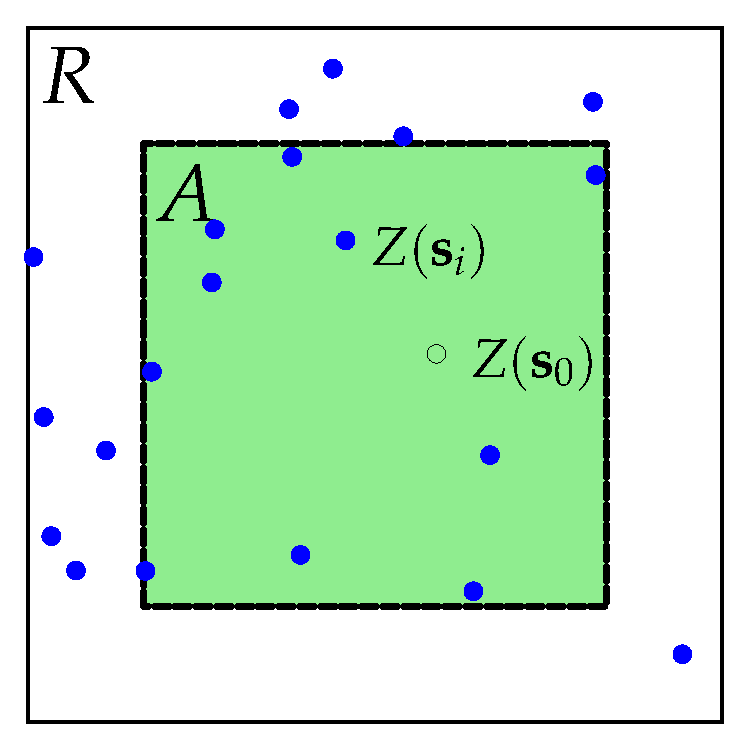
\includegraphics[width=4cm]{figure/BlockPred-plot} 
		\end{center} &
		\begin{itemize}
			\item $Z(A) \equiv \int_{A} Z(\bu) d\bu/|A|$
			\item $x_i(A) \equiv \int_{A} x_i(\bu) d\bu/|A|$ \\
			\item $\bx_A \equiv [x_1(A),\ldots,x_p(A)]\upp$ \\
			\item $\epsilon(A) \equiv \int_{A} \epsilon(\bu) d\bu/|A|$
		\end{itemize}

	\end{tabular}

	\[ 
		\left(\begin{array}{c}
		\bz \\ Z(A)
		\end{array}\right)	=
		\left(\begin{array}{c}
		\bX \\ \bx_A\upp
		\end{array}\right)\bbeta +
		\left(\begin{array}{c}
		\bepsilon \\ \epsilon(A)
		\end{array}\right)
	\]

\end{frame}

%-------------------------------------------------------------------------------
%                 Block Prediction
%-------------------------------------------------------------------------------

\begin{frame}[fragile]
\frametitle{Block Prediction}

	\begin{tabular} {p{3cm} p{6cm}}
		\begin{center}
			\vspace{-1cm}
			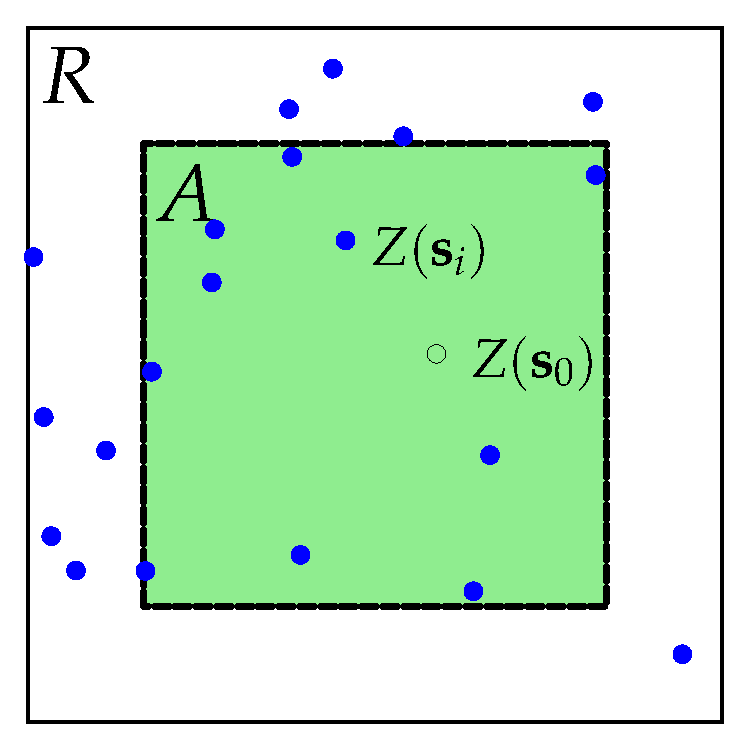
\includegraphics[width=3cm]{figure/BlockPred-plot} 
		\end{center} &
	\footnotesize
		\begin{itemize}
			\item $c_i(A) \equiv \cov(\epsilon(\bs_i),\epsilon(A)) = \int_{A} \cov(\epsilon(\bs_i), \epsilon(\bu)) d\bu/|A|$
			\item $\bc_A \equiv [c_1(A),\ldots,c_n(A)]$ \\
			\item $\sigma^2_A \equiv \int_{A}\int_{A} \cov(\epsilon(\bu), \epsilon(\bv)) d\bu d\bv /|A|^2$
		\end{itemize}

	\end{tabular} \\
	\footnotesize
	recall: $\cov(Y_1,Y_2 + Y_3) = \cov(Y_1,Y_2) + \cov(Y_1, Y_3)$ 
	\normalsize
	\[ 
		\cov\left(\begin{array}{c}
		\bepsilon \\ \epsilon(A)
		\end{array}\right) = 
		\left(\begin{array}{cc}
		\bSigma & \bc_A \\ \bc_A\upp & \sigma_A^2
		\end{array}\right)
	\]
\end{frame}

%-------------------------------------------------------------------------------
%                 Review of BLUP and Point Prediction
%-------------------------------------------------------------------------------

\begin{frame}[fragile]
\frametitle{Block Prediction}
	\vspace{-.5cm}
	\[
		\left(\begin{array}{c}
		\bz \\ Z(A)
		\end{array}\right)	=
		\left(\begin{array}{c}
		\bX \\ \bx_A\upp
		\end{array}\right)\bbeta +
		\left(\begin{array}{c}
		\bepsilon \\ \epsilon(A)
		\end{array}\right)
	\] \\
	\[ 
		\cov\left(\begin{array}{c}
		\bepsilon \\ \epsilon(A)
		\end{array}\right) = 
		\left(\begin{array}{cc}
		\bSigma & \bc_A \\ \bc_A\upp & \sigma_A^2
		\end{array}\right)
	\] \\
	Best Linear Unbiased Prediction (BLUP) \\
	minimize: $\cre{E(\blambda\upp\bz - Z(A))^2}$ subject to 	$\cre{E[\blambda\upp\bz] = E[Z(A)] \ \forall \ \bbeta}$ \\
	Unbiasedness $\Rightarrow \bX\upp\blambda = \bx_A $ \\		
	$E[\blambda\upp\bepsilon\bepsilon\upp\blambda - 2\blambda\upp\bepsilon \epsilon(A) + \epsilon(A)^2] = \blambda\upp\bSigma\blambda - 2\blambda\upp\bc_A + \sigma_A^2$ \\
	$\blambda = \bSigma\upi(\bc_A + \bX(\bX\upp\bSigma\upi\bX)\upi(\bx_A - \bX\upp\bSigma\upi\bc_A))$ \\

	$ \cre{\hat{Z}(A) = \blambda\upp\bz}, \quad \cre{\var(\hat{Z}(A)) = \blambda\upp\bSigma\blambda - 2\blambda\upp\bc_A + \sigma_A^2}$

\end{frame}

%-------------------------------------------------------------------------------
%                 Alternative Formulas
%-------------------------------------------------------------------------------

\begin{frame}[fragile]
\frametitle{Alternative Formulas}

	\begin{center}
		$\hat{Z}(A) = \blambda\upp\bz = \bc_A\upp\bSigma\upi(\bz - \hat{\bmu}) + \hat{\bmu}_A$
	\end{center} \\
	where \\
	\begin{center}
		$\hat{\bmu} = \bX\hat{\bbeta}_{GLS} \quad \hat{\bmu}_A = \bx_A\upp\hat{\bbeta}_{GLS} \quad 
\hat{\bbeta}_{GLS} = (\bX\upp\bSigma\upi\bX)\upi\bX\upp\bSigma\upi\bz$
	\end{center} \\
	and \\
	\begin{center}
		$E(\blambda\upp\bz - Z(A))^2 = \sigma_A^2 - \bc_A\upp\bSigma\upi\bc_A + \bd_A\upp(\bX\upp\bSigma\upi\bX)\upi\bd_A$
	\end{center} \\
	where \\
	\begin{center}
		$\bd_A = \bx_A - \bX\upp\bSigma\upi\bc_A$
	\end{center} 
	


\end{frame}

%-------------------------------------------------------------------------------
%                 Simulations
%-------------------------------------------------------------------------------

\section{Simulations}
\subsection{}
\begin{frame}[fragile]
\frametitle{Fixed Pattern, Random Samples}
\vspace{-.3cm}
\tiny
Ver Hoef, J.M.  2002.  Sampling and geostatistics for spatial data.  {\it Ecoscience} {\bf 9}: 152 - 161.\\
\vspace{.3cm}
	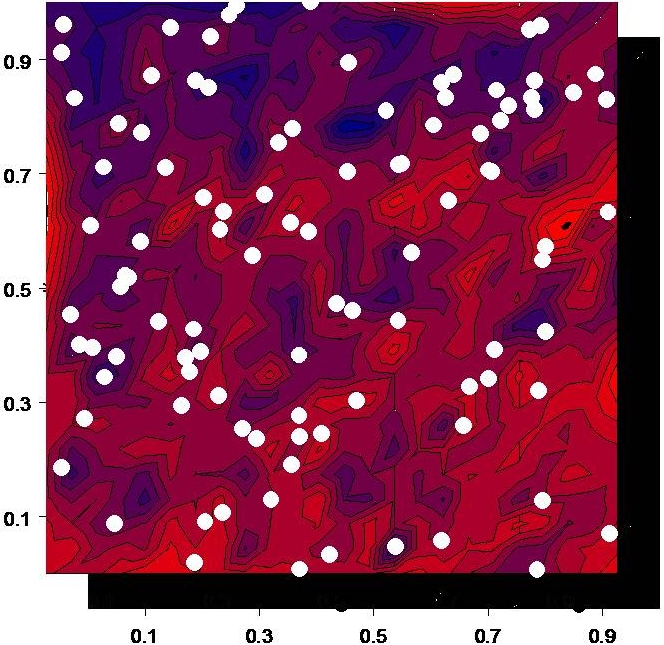
\includegraphics[width=.5\maxwidth]{figure/fixedPatternRandSamp1.jpg}
	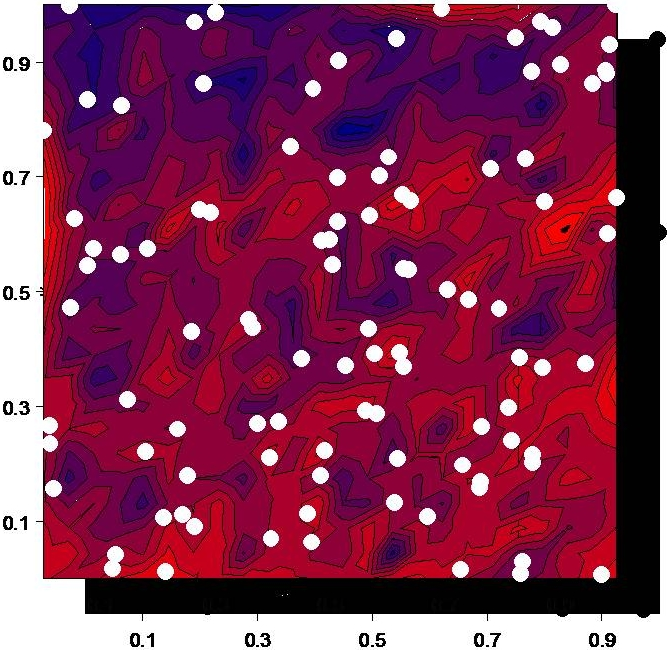
\includegraphics[width=.5\maxwidth]{figure/fixedPatternRandSamp2.jpg}

\end{frame}

%-------------------------------------------------------------------------------
%                 Simulations
%-------------------------------------------------------------------------------

\begin{frame}[fragile]
\frametitle{Fixed Pattern, Random Samples}

1000 random samples of size 100 \\
\footnotesize
	\begin{table}[ht]
	\centering
	\begin{tabular}{ccc}
	Validation Statistics & Simple Random Sample & Block Prediction \\ 
	\cbl{Bias} & \cre{0.002} & \cre{-0.020} \\ 
	\cbl{RMSPE} & \cre{1.28} & \cre{1.02} \\ 
	\cbl{RAEV} & \cre{1.29} & \cre{1.00} \\ 
	\cbl{80\%CI} & \cre{0.813} & \cre{0.806} \\ 
	\end{tabular}
	\end{table}

\end{frame}


%-------------------------------------------------------------------------------
%                 Ozone Example
%-------------------------------------------------------------------------------

\section{Examples}
\subsection{}
\begin{frame}[fragile]
\frametitle{Ozone Example}




	\begin{tabular} {p{4.5cm} p{4.5cm}}
		\vspace{.1cm}
		\begin{center}
			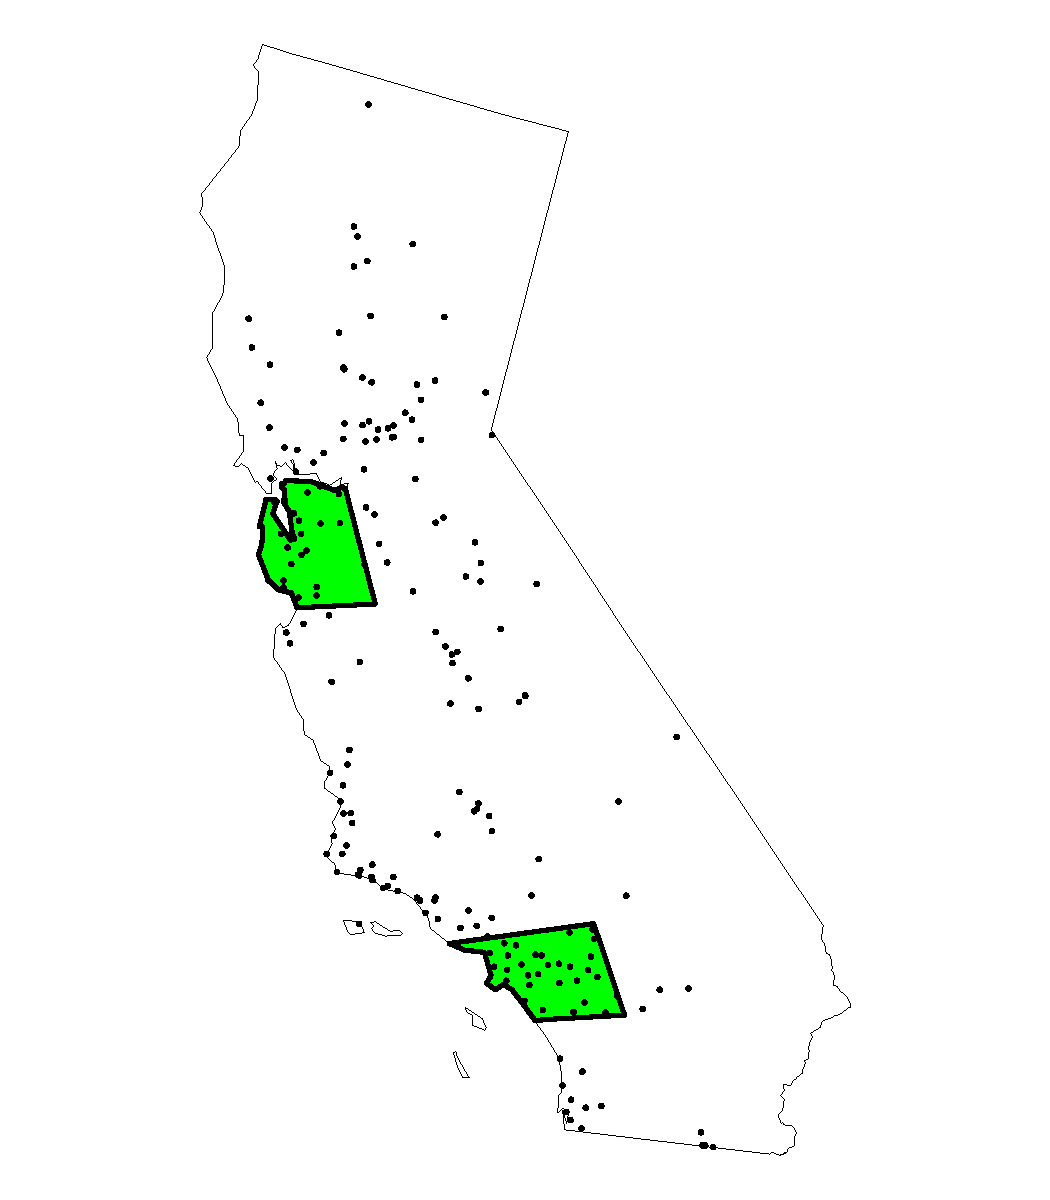
\includegraphics[width = \maxwidth]{figure/CApolys-plot} 
		\end{center} &
		\vspace{-.7cm}
		\begin{center}
			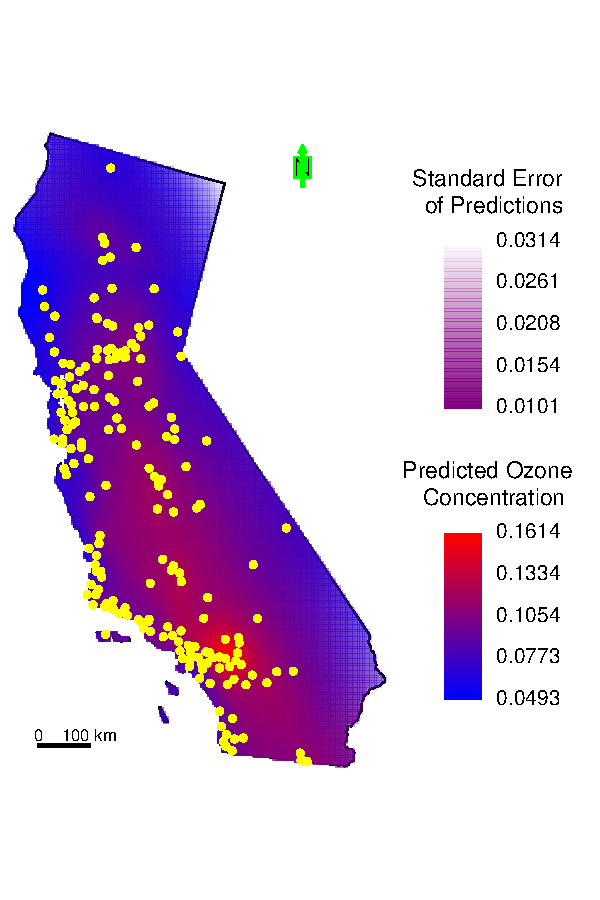
\includegraphics[width = \maxwidth]{figure/CA-predMap} 
		\end{center}
	\end{tabular}

\end{frame}

%-------------------------------------------------------------------------------
%                 Ozone Example
%-------------------------------------------------------------------------------

\begin{frame}[fragile]
\frametitle{Ozone Example}

\begin{knitrout}\tiny
\definecolor{shadecolor}{rgb}{0.969, 0.969, 0.969}\color{fgcolor}\begin{kframe}
\begin{alltt}
\hlfunctioncall{library}(spPlotSampCourse)
\hlfunctioncall{library}(maptools)
path <- \hlfunctioncall{system.file}(\hlstring{"rawdata/airPolluteCA"}, package = \hlstring{"spPlotSampCourse"})
outlineFile <- \hlfunctioncall{paste}(path, \hlstring{"/"}, \hlstring{"ca_outline"}, sep = \hlstring{""})
otl <- \hlfunctioncall{readShapePoly}(outlineFile)
pointsFile <- \hlfunctioncall{paste}(path, \hlstring{"/"}, \hlstring{"ca_ozone_pts"}, sep = \hlstring{""})
pts <- \hlfunctioncall{readShapePoints}(pointsFile)
polyLAFile <- \hlfunctioncall{paste}(path, \hlstring{"/"}, \hlstring{"polyLA"}, sep = \hlstring{""})
polyLA <- \hlfunctioncall{readShapePoly}(polyLAFile)
polySFFile <- \hlfunctioncall{paste}(path, \hlstring{"/"}, \hlstring{"polySF"}, sep = \hlstring{""})
polySF <- \hlfunctioncall{readShapePoly}(polySFFile)
ozFit1 <- \hlfunctioncall{splmm}(OZONE ~ 1, spdata = pts, estMeth = \hlstring{"REML"}, varComps = \hlstring{"circular"}, 
    useAnisotropy = TRUE)
blockPredGridLA <- \hlfunctioncall{createBlockPredGrid}(polyLA)
\hlfunctioncall{predictBlock}(ozFit1, blockPredGridLA)
\end{alltt}
\begin{verbatim}
##    OZONE BlockPredSE
## 1 0.1256     0.00178
\end{verbatim}
\begin{alltt}
blockPredGridSF <- \hlfunctioncall{createBlockPredGrid}(polySF)
\hlfunctioncall{predictBlock}(ozFit1, blockPredGridSF)
\end{alltt}
\begin{verbatim}
##     OZONE BlockPredSE
## 1 0.08856    0.002618
\end{verbatim}
\end{kframe}
\end{knitrout}


\end{frame}

%-------------------------------------------------------------------------------
%                 Meuse Example
%-------------------------------------------------------------------------------

\begin{frame}[fragile]
\frametitle{Meuse Example}

	






	\begin{tabular} {p{3cm} p{3cm} p{3cm}}
		\vspace{-.5cm}
		\begin{center}
			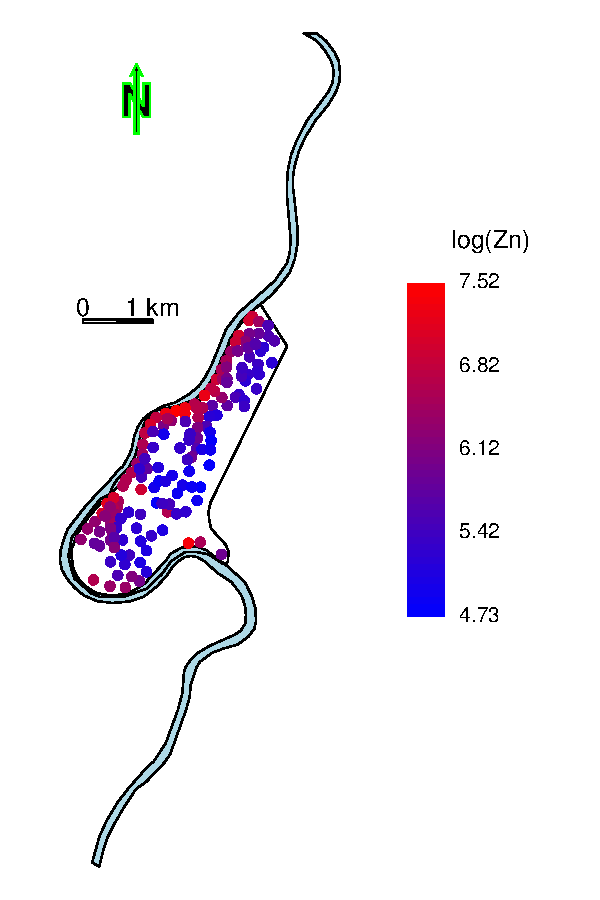
\includegraphics[width = 4cm]{figure/colorPointsMeuseLogZN-plot}
		\end{center}  &
		\vspace{1cm}	
		\begin{center}
			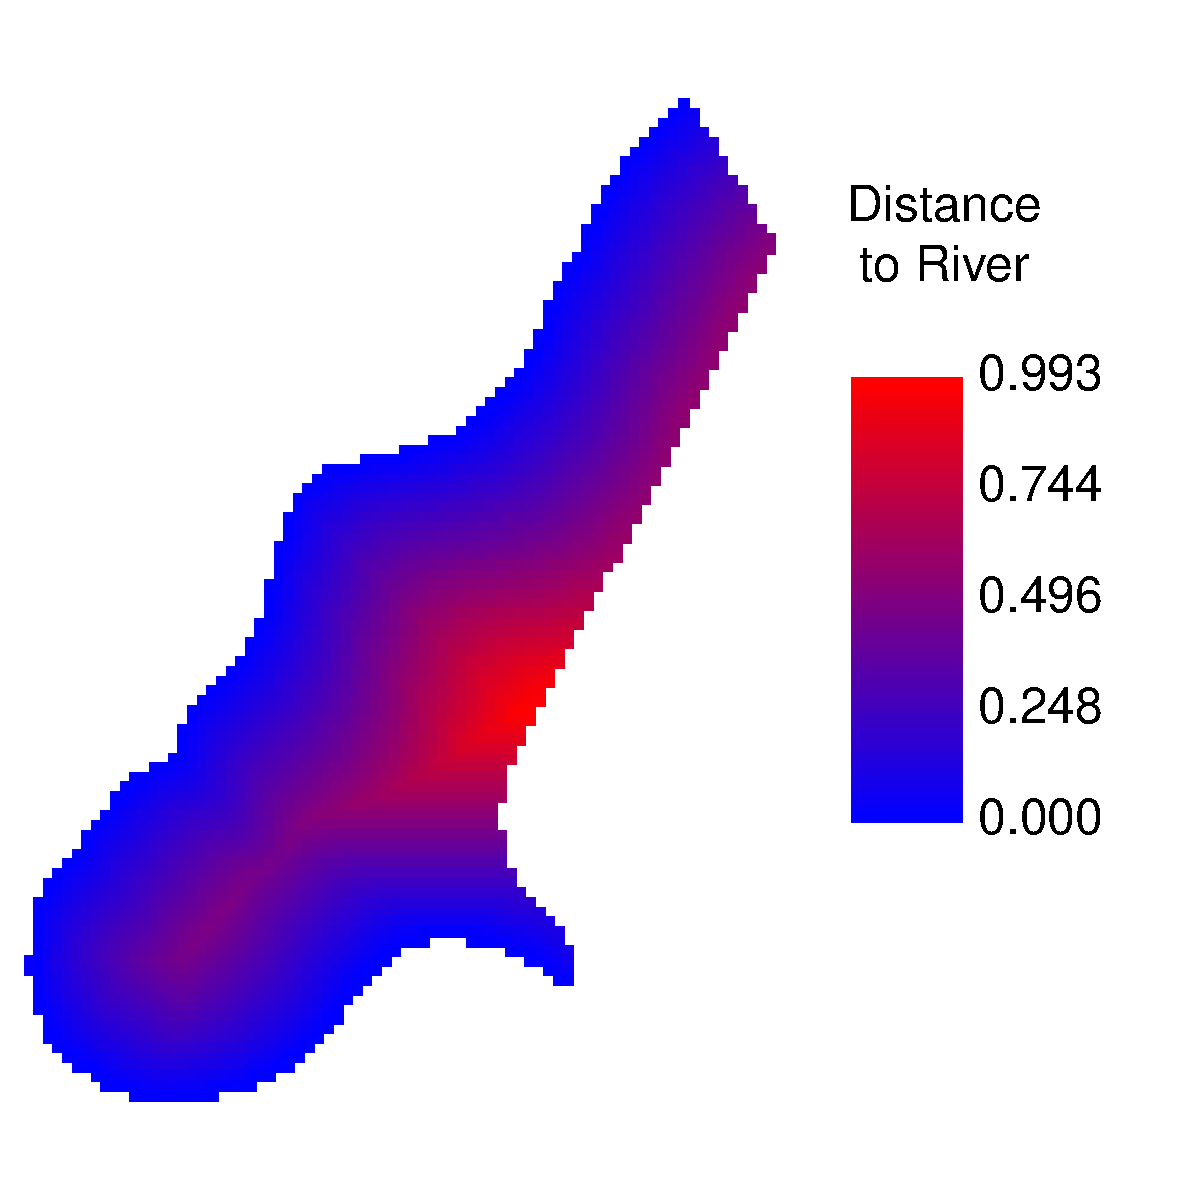
\includegraphics[width = 3cm]{figure/meuseDist-plot}
		\end{center}  &
		\vspace{1cm}
		\begin{center}
			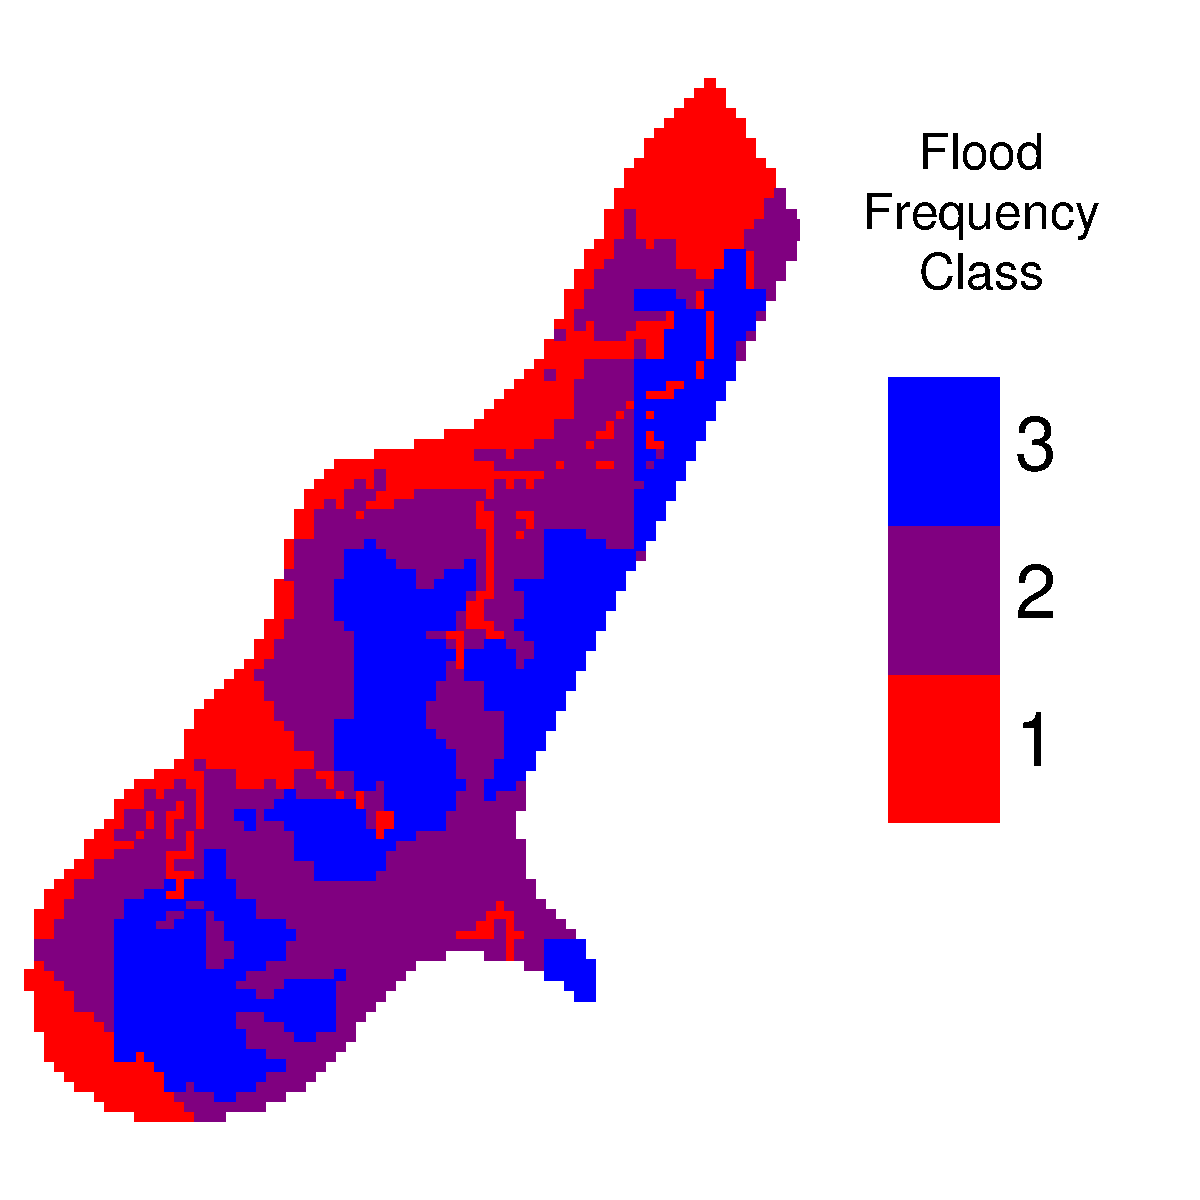
\includegraphics[width = 3cm]{figure/meuseFFreq-plot} 
		\end{center}
	\end{tabular}

\end{frame}

%-------------------------------------------------------------------------------
%                 Meuse Example
%-------------------------------------------------------------------------------

\begin{frame}[fragile]
\frametitle{Meuse Example}

\begin{knitrout}\tiny
\definecolor{shadecolor}{rgb}{0.969, 0.969, 0.969}\color{fgcolor}\begin{kframe}
\begin{alltt}
\hlfunctioncall{data}(meuse)
\hlfunctioncall{coordinates}(meuse) <- ~x + y
\hlfunctioncall{proj4string}(meuse) <- \hlfunctioncall{CRS}(\hlstring{"+init=epsg:28992"})
\hlfunctioncall{data}(meuse.grid)
\hlfunctioncall{coordinates}(meuse.grid) <- ~x + y
\hlfunctioncall{proj4string}(meuse.grid) <- \hlfunctioncall{CRS}(\hlstring{"+init=epsg:28992"})
znFit1 <- \hlfunctioncall{splmm}(zinc ~ dist + ffreq, spdata = meuse, varComps = \hlstring{"besselK"})
\hlfunctioncall{predictBlock}(znFit1, meuse.grid)
\end{alltt}
\begin{verbatim}
##    zinc BlockPredSE
## 1 351.9       18.73
\end{verbatim}
\end{kframe}
\end{knitrout}


\end{frame}

%-------------------------------------------------------------------------------
%                 Meuse Example
%-------------------------------------------------------------------------------

\begin{frame}[fragile]
\frametitle{Meuse Example}

\begin{knitrout}\tiny
\definecolor{shadecolor}{rgb}{0.969, 0.969, 0.969}\color{fgcolor}\begin{kframe}
\begin{alltt}
\hlfunctioncall{summary}(znFit1)$coefficients
\end{alltt}
\begin{verbatim}
##             Estimate Std. Error t value  Pr(>|t|)
## (Intercept)    959.9      93.87  10.225 5.620e-19
## dist         -1189.6     234.71  -5.068 1.159e-06
## ffreq2        -288.7      37.26  -7.748 1.262e-12
## ffreq3        -276.1      57.92  -4.766 4.371e-06
\end{verbatim}
\begin{alltt}
\hlfunctioncall{summary}(znFit1)$covparms
\end{alltt}
\begin{verbatim}
##   Variance Component Parameter Type  Estimate
## 1             nugget         nugget 7.858e+03
## 2            besselK         parsil 8.486e+04
## 3            besselK          range 8.250e+02
## 4            besselK         extrap 7.807e-01
\end{verbatim}
\begin{alltt}
\hlfunctioncall{summary}(znFit1)$R2g
\end{alltt}
\begin{verbatim}
## [1] 0.3965
\end{verbatim}
\end{kframe}
\end{knitrout}


\end{frame}


\end{document}
